\documentclass[aspectratio=169,10pt]{beamer}
% Shared Beamer style for MA 25-31018 Persamaan Diferensial Parsial
\usepackage[utf8]{inputenc}
\usepackage[T1]{fontenc}
\usepackage{lmodern}
\usepackage{amsmath,amssymb,mathtools,bm}
\usepackage{graphicx}
\usepackage{booktabs,array}
\usepackage{listings}
\usepackage{xcolor}
\usepackage{tikz}
\usetikzlibrary{calc,positioning,decorations.pathreplacing}

\definecolor{pdpNavy}{HTML}{0F172A}
\definecolor{pdpTeal}{HTML}{0F766E}
\definecolor{pdpMint}{HTML}{CCFBF1}
\definecolor{pdpAmber}{HTML}{F59E0B}
\definecolor{pdpSlate}{HTML}{334155}
\definecolor{pdpBg}{HTML}{F8FAFC}
\definecolor{pdpLine}{HTML}{CBD5E1}
\definecolor{pdpSoftTeal}{HTML}{ECFDF5}
\definecolor{pdpSoftAmber}{HTML}{FFF7ED}

\setbeamercolor{normal text}{fg=pdpNavy,bg=pdpBg}
\setbeamercolor{frametitle}{fg=pdpNavy,bg=pdpBg}
\setbeamercolor{title}{fg=pdpNavy}
\setbeamercolor{subtitle}{fg=pdpTeal}
\setbeamercolor{block title}{fg=white,bg=pdpTeal}
\setbeamercolor{block body}{fg=pdpNavy,bg=white}
\setbeamercolor{alerted text}{fg=pdpAmber!85!black}
\setbeamerfont{title}{series=\bfseries,size=\Large}
\setbeamerfont{frametitle}{series=\bfseries,size=\large}
\setbeamerfont{block title}{series=\bfseries}
\setbeamertemplate{navigation symbols}{}
\setbeamertemplate{itemize item}{\color{pdpTeal}$\blacktriangleright$}
\setbeamertemplate{itemize subitem}{\color{pdpAmber}$\bullet$}
\setbeamersize{text margin left=.65cm,text margin right=.65cm}

\newcommand{\pdpfooter}[2]{%
\setbeamertemplate{footline}{%
  \leavevmode\hbox{%
  \begin{beamercolorbox}[wd=.34\paperwidth,ht=2.55ex,dp=1.05ex,leftskip=.65cm]{author in head/foot}%
    \scriptsize Tim Pengajar PDP
  \end{beamercolorbox}%
  \begin{beamercolorbox}[wd=.40\paperwidth,ht=2.55ex,dp=1.05ex,center]{title in head/foot}%
    \scriptsize #1
  \end{beamercolorbox}%
  \begin{beamercolorbox}[wd=.26\paperwidth,ht=2.55ex,dp=1.05ex,rightskip=.65cm plus1fil]{date in head/foot}%
    \scriptsize Rifky Fauzi\hfill\insertframenumber/\inserttotalframenumber
  \end{beamercolorbox}}\vskip0pt% 
}}

\newcommand{\pdporangeline}{\vspace{0.15em}\textcolor{pdpAmber}{\rule{0.9cm}{1.3pt}}\vspace{0.35em}}
\newcommand{\pdpnote}[1]{{\scriptsize\color{pdpSlate}#1}}
\newcommand{\pdpkey}[1]{\textbf{\color{pdpTeal}#1}}
\newcommand{\pdpsource}[1]{{\fontsize{5.5}{6.2}\selectfont\color{pdpSlate}#1}}
\newcommand{\pdppill}[1]{\tikz[baseline=(X.base)]\node[fill=pdpMint,draw=pdpTeal,rounded corners=3pt,inner xsep=5pt,inner ysep=2pt](X){\scriptsize\bfseries #1};}

\lstdefinestyle{matlab}{
  language=Matlab,
  basicstyle=\ttfamily\scriptsize,
  keywordstyle=\color{pdpTeal}\bfseries,
  commentstyle=\color{pdpSlate},
  stringstyle=\color{pdpAmber!80!black},
  showstringspaces=false,
  breaklines=true,
  frame=single,
  framerule=0.4pt,
  rulecolor=\color{pdpLine},
  backgroundcolor=\color{white},
  xleftmargin=1mm,
  xrightmargin=1mm
}

\pdpfooter{PDP Orde 1 - Case-Based Project}{}

\title{Pendekatan Numerik PDP Orde 1}
\subtitle{Case: Polutan Sungai dan Kepadatan Koridor Gedung}
\author{Tim Pengajar Persamaan Diferensial Parsial}
\institute{Program Studi Matematika - Institut Teknologi Sumatera}
\date{Minggu 6}

\begin{document}

\begin{frame}[plain]
  \begin{tikzpicture}[remember picture,overlay]
    \fill[pdpNavy] (current page.south west) rectangle ([xshift=0.33\paperwidth]current page.north west);
    \fill[pdpTeal] ([xshift=0.33\paperwidth]current page.south west) rectangle ([xshift=0.337\paperwidth]current page.north west);
  \end{tikzpicture}
  \vspace{0.7cm}
  \begin{columns}[T]
    \column{0.30\textwidth}
      \color{white}
      {\bfseries MA 25-31018}\par\vspace{0.25cm}
      {\Large\bfseries PERSAMAAN\\ DIFERENSIAL\\ PARSIAL}\par\vspace{1.0cm}
      {\color{pdpMint}\large\bfseries Minggu 6}
    \column{0.64\textwidth}
      {\Huge\bfseries Pendekatan Numerik PDP Orde 1}\par
      \pdporangeline
      {\Large Case: Polutan Sungai dan Kepadatan Koridor Gedung}\par\vspace{0.75cm}
      {\bfseries Tim Pengajar Persamaan Diferensial Parsial}\par\vspace{1.0cm}
      Program Studi Matematika\par
      Institut Teknologi Sumatera\par\vfill
      {\scriptsize Footer: Rifky Fauzi}
  \end{columns}
\end{frame}

\begin{frame}{Arah Minggu 6: dari karakteristik ke simulasi}
\begin{columns}[T]
\column{0.55\textwidth}
\begin{block}{Jembatan analitik - numerik}
Sebelumnya kita memakai karakteristik untuk membaca lintasan informasi. Minggu ini lintasan itu dijadikan dasar untuk membangun skema beda hingga.
\end{block}
\vspace{0.4em}
\begin{itemize}
  \item Model utama: transport/adveksi satu dimensi.
  \item Fokus: skema upwind, visualisasi, dan interpretasi hasil.
  \item CFL dibahas singkat sebagai syarat agar simulasi masuk akal.
\end{itemize}
\column{0.40\textwidth}
\centering
\vspace{0.3cm}
\pdppill{model nyata}\hspace{0.35cm}\pdppill{PDP orde 1}\par\vspace{0.55cm}
\pdppill{beda hingga}\hspace{0.35cm}\pdppill{hasil visual}\par\vspace{0.7cm}
\begin{block}{Output yang dikejar}
Bukan hanya angka, tetapi cerita: kapan puncak terjadi, di mana lokasinya, dan apa konsekuensinya.
\end{block}
\end{columns}
\end{frame}

\begin{frame}{Case 1: Polutan sepanjang sungai}
\begin{columns}[T]
\column{0.53\textwidth}
\begin{block}{Situasi nyata}
Terjadi pelepasan polutan di hulu sungai. Arus sungai membawa polutan ke hilir, sambil konsentrasinya menurun karena proses degradasi alami.
\end{block}
\vspace{0.2em}
\begin{itemize}
  \item $x$: jarak dari hulu (km), $t$: waktu (jam)
  \item $C(x,t)$: konsentrasi polutan (mg/L)
  \item $v$: kecepatan aliran sungai
  \item $k$: laju peluruhan/degradasi
\end{itemize}
\column{0.42\textwidth}
\begin{block}{Model PDP orde 1}
\[
  C_t + v C_x = -k C,\qquad v>0.
\]
\end{block}
\begin{block}{Solusi karakteristik}
\[
  \frac{dx}{dt}=v,\qquad \frac{dC}{dt}=-kC,
\]
\[
  C(x,t)=C_0(x-vt)e^{-kt}.
\]
\end{block}
\end{columns}
\end{frame}

\begin{frame}{Beda hingga upwind untuk polutan}
\begin{columns}[T]
\column{0.51\textwidth}
\begin{block}{Grid}
\[
  x_i=i\Delta x,\qquad t^n=n\Delta t,
  \qquad C_i^n\approx C(x_i,t^n).
\]
\end{block}
\begin{block}{Skema eksplisit}
Untuk aliran ke kanan, $v>0$:
\[
C_i^{n+1}
= C_i^n
-\lambda(C_i^n-C_{i-1}^n)
-k\Delta t\, C_i^n,
\qquad
\lambda=\frac{v\Delta t}{\Delta x}.
\]
\end{block}
\column{0.44\textwidth}
\begin{block}{CFL singkat}
Untuk adveksi eksplisit upwind:
\[
\boxed{0\leq \lambda \leq 1.}
\]
Interpretasi: dalam satu langkah waktu, informasi tidak boleh melompat lebih dari satu sel grid.
\end{block}
\begin{block}{Parameter simulasi}
\[
L=10\text{ km},\quad v=2\text{ km/jam},\quad k=0.25\text{ jam}^{-1}
\]
\[
\Delta x=0.02,\quad \Delta t=0.006,\quad \lambda=0.6.
\]
\end{block}
\end{columns}
\end{frame}

\begin{frame}[fragile]{Simulasi MATLAB: inti algoritma}
\begin{columns}[T]
\column{0.56\textwidth}
\begin{lstlisting}[style=matlab]
for n = 1:Nt
    Cn = C;
    C(2:end) = Cn(2:end) ...
        - lam*(Cn(2:end)-Cn(1:end-1)) ...
        - k*dt*Cn(2:end);
    C(1) = 0;          % batas hulu
    C = max(C,0);
end
\end{lstlisting}
\column{0.39\textwidth}
\begin{block}{Yang disimpan}
\begin{itemize}
  \item profil $C(x,t)$ pada beberapa waktu;
  \item heatmap $x$-$t$;
  \item kurva sensor $C(x_s,t)$;
  \item waktu puncak dan konsentrasi maksimum.
\end{itemize}
\end{block}
\begin{block}{Catatan numerik}
Upwind stabil, tetapi cenderung memberi \alert{difusi numerik}: puncak menjadi lebih rendah dan profil melebar.
\end{block}
\end{columns}
\end{frame}

\begin{frame}{Hasil polutan: profil dan peta ruang-waktu}
\begin{columns}[T]
\column{0.52\textwidth}
\centering
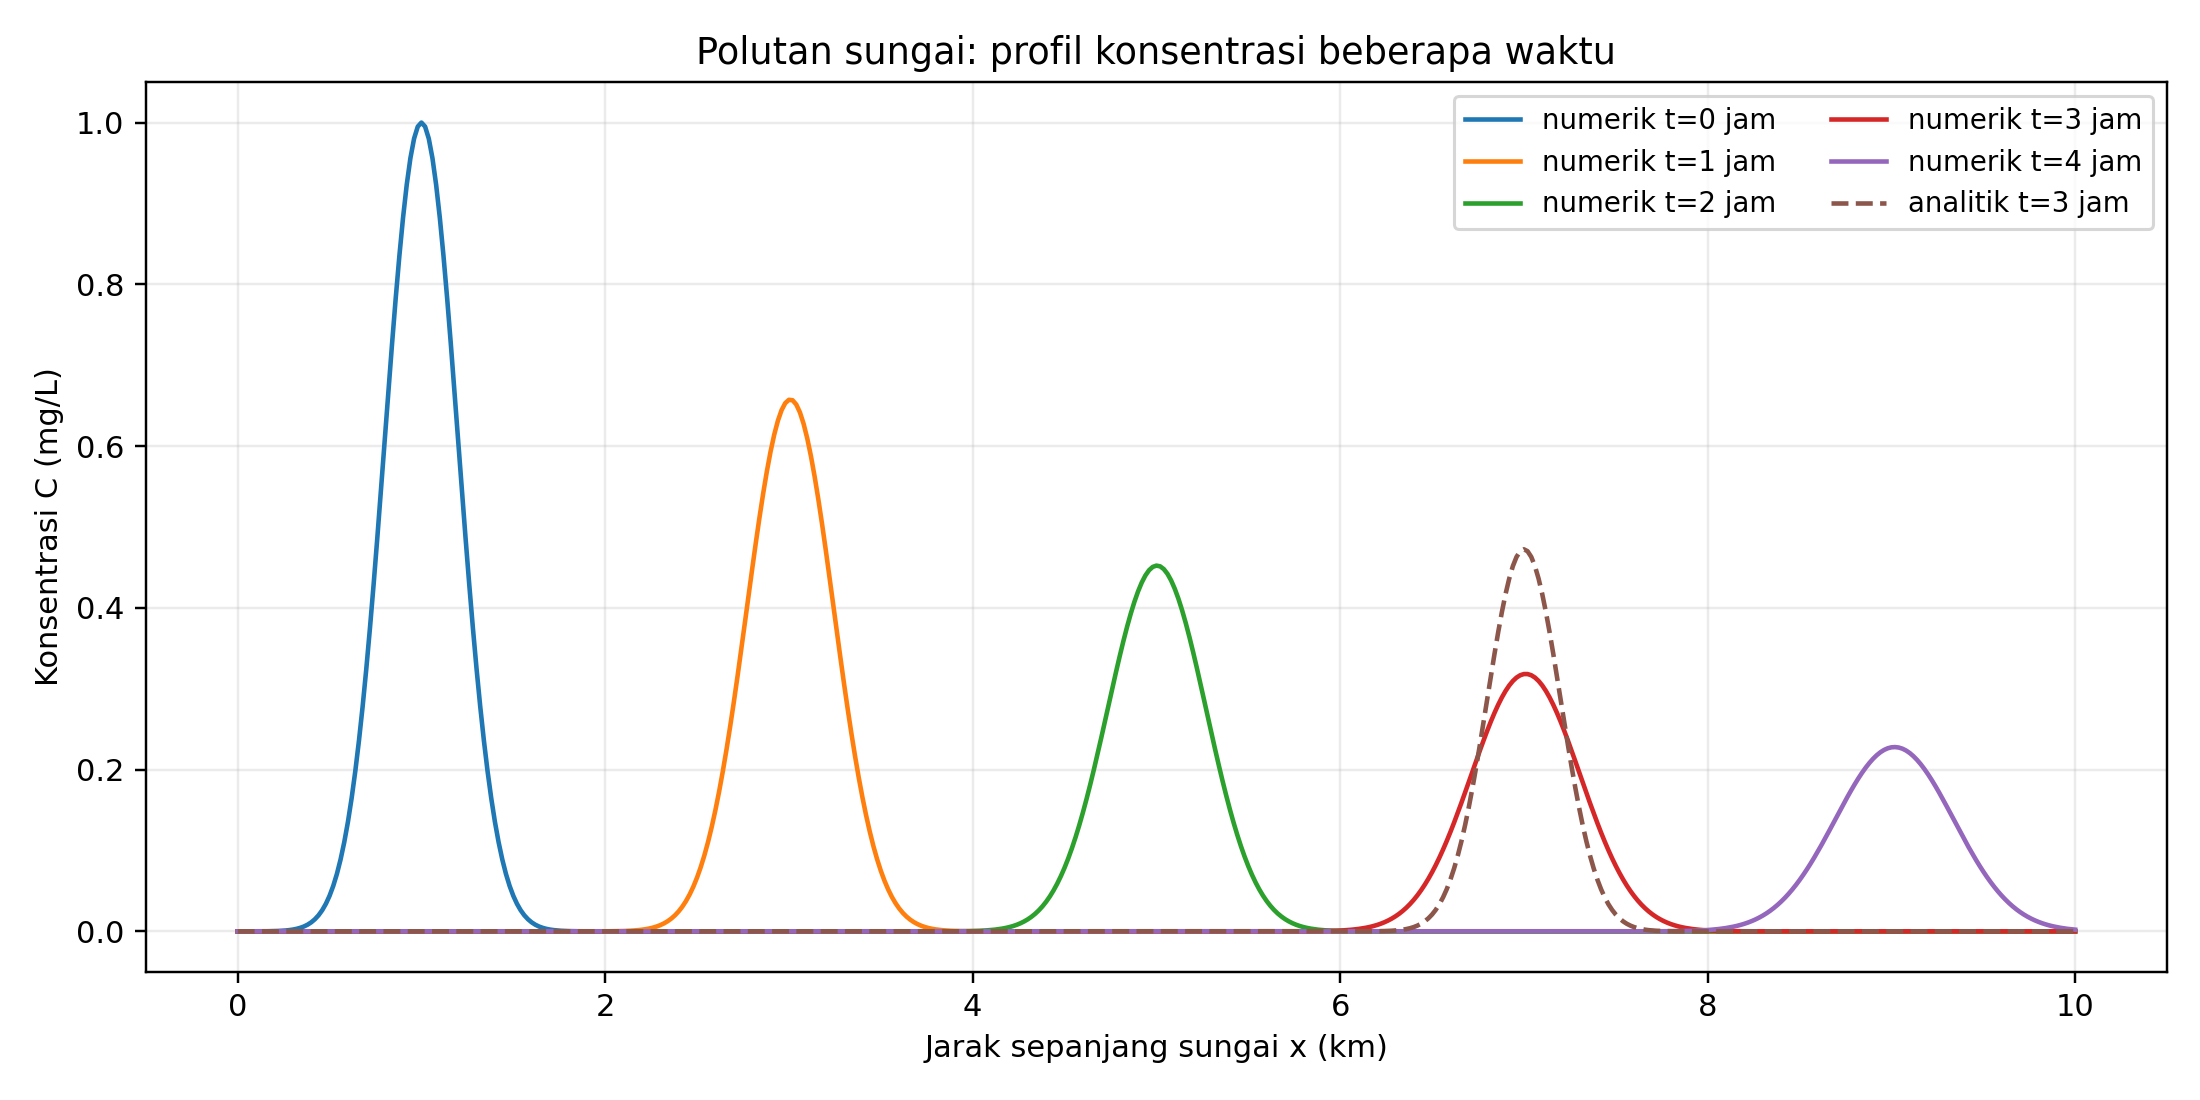
\includegraphics[width=\linewidth]{figures/pollutant_profiles.png}
\column{0.43\textwidth}
\centering
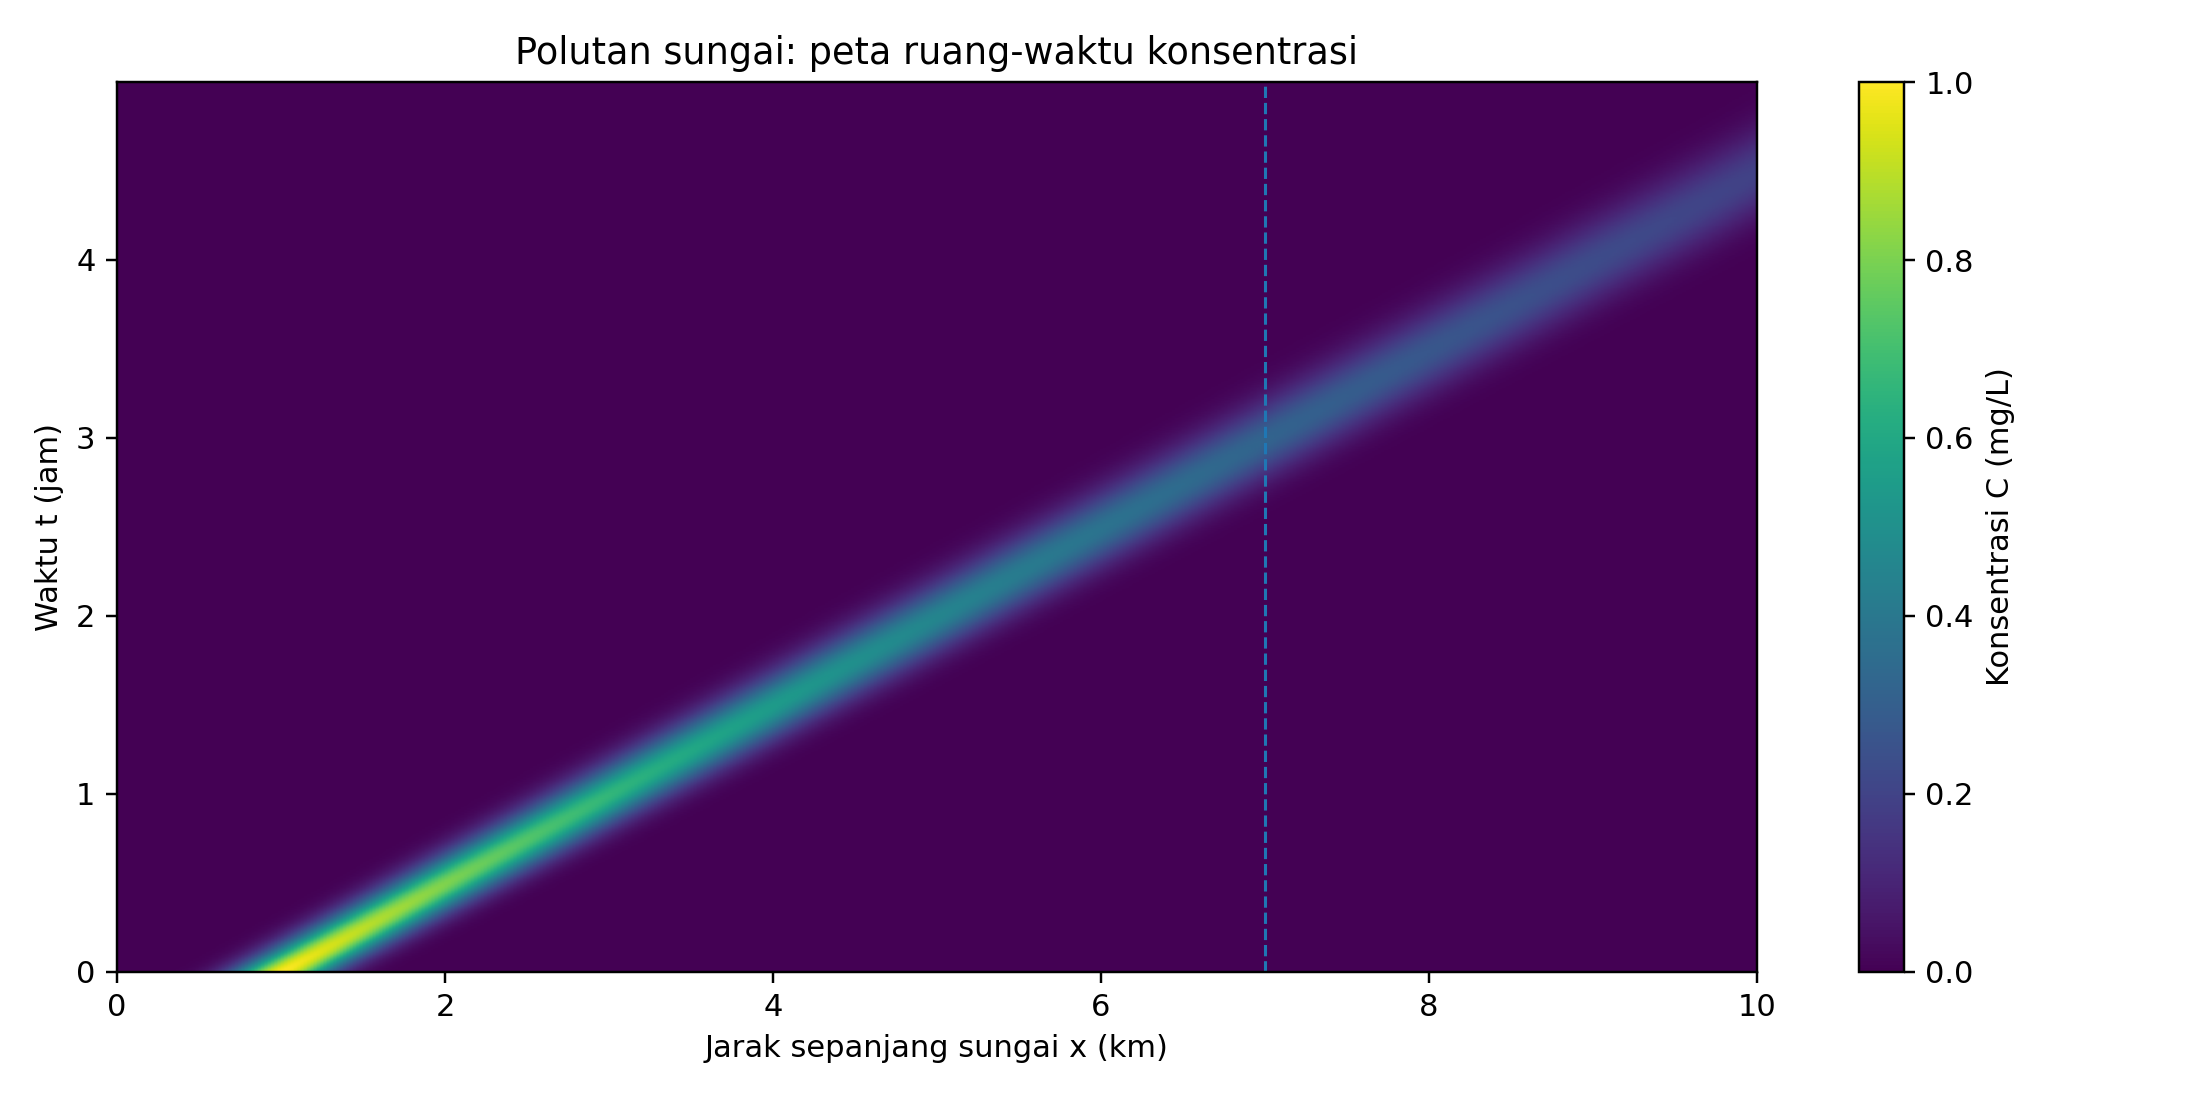
\includegraphics[width=\linewidth]{figures/pollutant_heatmap.png}
\vspace{0.2em}
\begin{block}{Cara membaca gambar}
\small
\begin{itemize}
  \item Pulsa bergerak ke hilir mengikuti arus.
  \item Puncak turun karena degradasi dan difusi numerik.
  \item Sensor $x=7$ km: puncak $\approx2.99$ jam, $C\approx0.319$ mg/L.
\end{itemize}
\end{block}
\end{columns}
\end{frame}

\begin{frame}{Penyajian hasil Case Polutan}
\begin{columns}[T]
\column{0.42\textwidth}
\centering
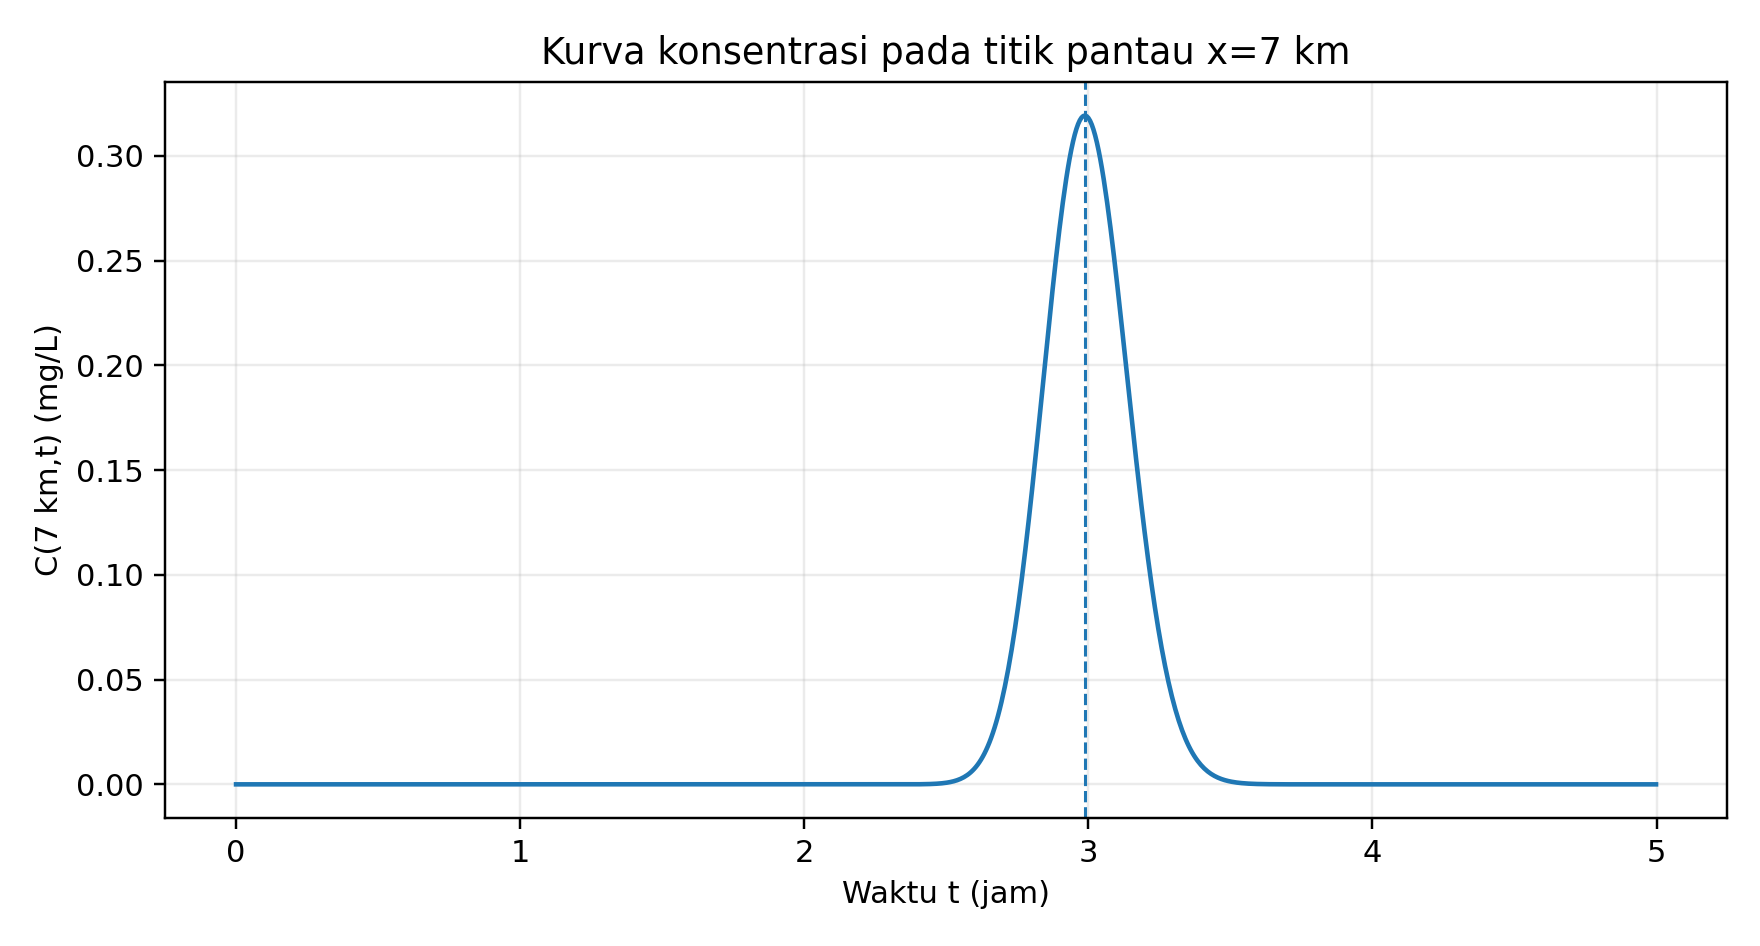
\includegraphics[width=\linewidth]{figures/pollutant_sensor.png}
\column{0.53\textwidth}
\begin{block}{Pertanyaan laporan}
\begin{itemize}
  \item Kapan polutan mencapai titik pantau?
  \item Berapa konsentrasi maksimum di titik tersebut?
  \item Bagaimana perubahan $\Delta x$ dan $\Delta t$ mempengaruhi hasil?
  \item Apa perbedaan profil numerik dengan solusi karakteristik?
\end{itemize}
\end{block}
\begin{block}{Kesimpulan sementara}
Skema beda hingga mengubah model analitik menjadi simulasi praktis: grafik sensor membantu menentukan waktu pemantauan, peringatan, atau penutupan intake air.
\end{block}
\end{columns}
\end{frame}

\begin{frame}{Case 2: Kepadatan mahasiswa di koridor gedung}
\begin{columns}[T]
\column{0.53\textwidth}
\begin{block}{Situasi nyata}
Beberapa ruang kelas bubar dan mahasiswa masuk ke satu koridor menuju pintu keluar. Kepadatan tinggi menurunkan kecepatan berjalan.
\end{block}
\begin{block}{Model conservation law dengan sumber}
\[
  \rho_t + \bigl(q(\rho)\bigr)_x = S(x,t),
\]
\[
  q(\rho)=\rho v(\rho),\qquad
  v(\rho)=v_{\max}\left(1-\frac{\rho}{\rho_{\max}}\right).
\]
\end{block}
\column{0.42\textwidth}
\begin{block}{Makna variabel}
\begin{itemize}
  \item $\rho(x,t)$: kepadatan mahasiswa di koridor.
  \item $q(\rho)$: arus orang per satuan lebar.
  \item $S(x,t)$: mahasiswa keluar dari ruang kelas.
  \item Boundary kanan: kapasitas pintu keluar.
\end{itemize}
\end{block}
\begin{block}{Diskritisasi konservatif}
\[
\rho_i^{n+1}=\rho_i^n-\frac{\Delta t}{\Delta x}
\left(F_{i+1/2}^n-F_{i-1/2}^n\right)+\Delta t\,S_i^n.
\]
\end{block}
\end{columns}
\end{frame}

\begin{frame}{Hasil evakuasi: heatmap dan kurva keluar}
\begin{columns}[T]
\column{0.48\textwidth}
\centering
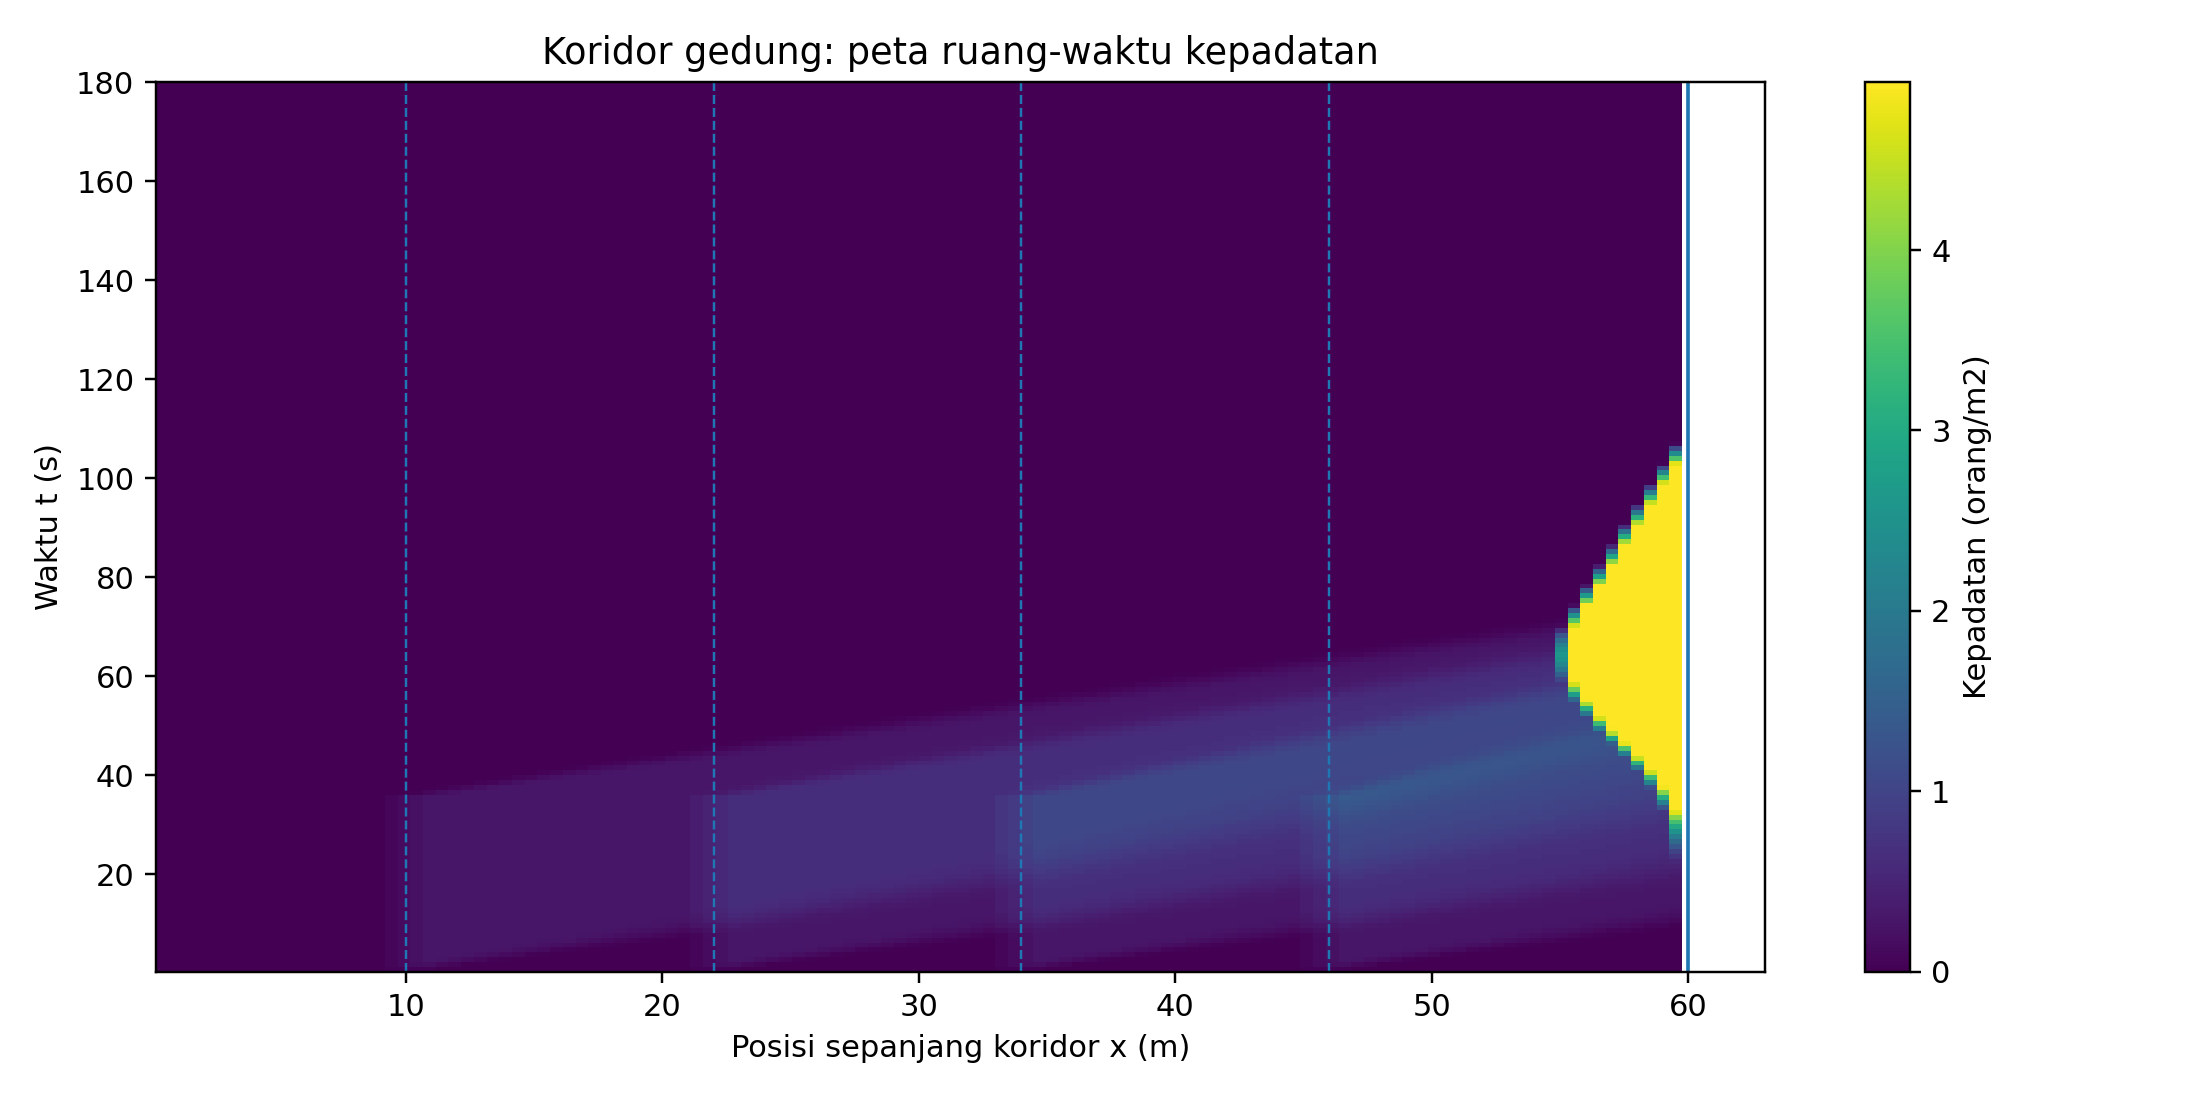
\includegraphics[width=\linewidth]{figures/evacuation_heatmap.png}
\column{0.48\textwidth}
\centering
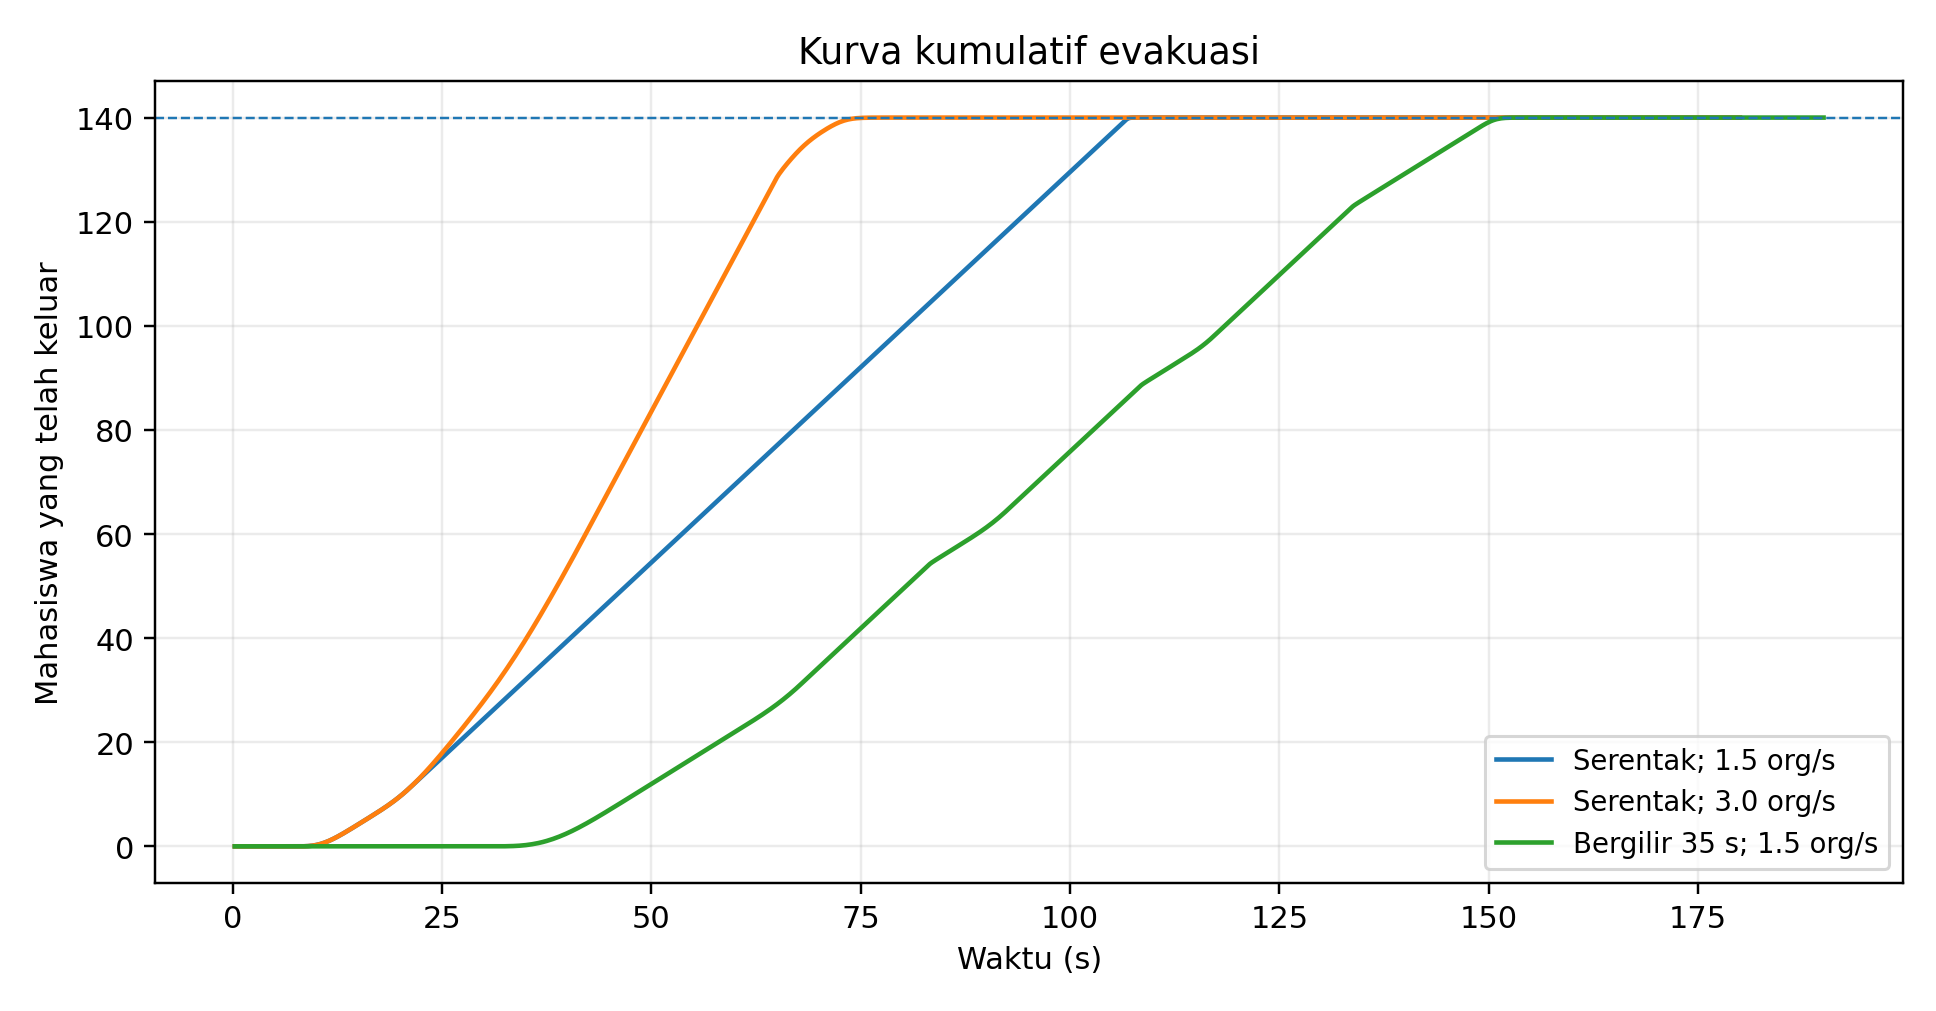
\includegraphics[width=\linewidth]{figures/evacuation_curves.png}
\vspace{0.2em}
\begin{block}{Ringkasan numerik}
\scriptsize
\begin{tabular}{p{0.44\linewidth}rr}
\toprule
Skenario & $\rho_{\max}$ & $t_{99}$ \\
\midrule
Serentak, pintu 1.5 org/s & 4.93 & 106 s \\
Serentak, pintu 3.0 org/s & 3.35 & 72 s \\
Bergilir 35 s, pintu 1.5 org/s & 3.05 & 150 s \\
\bottomrule
\end{tabular}
\end{block}
\end{columns}
\end{frame}

\begin{frame}{Simpulan untuk Case-Based Project}
\begin{columns}[T]
\column{0.54\textwidth}
\begin{block}{Pesan matematis}
\begin{itemize}
  \item PDP orde 1 memodelkan perpindahan informasi/massa/orang.
  \item Karakteristik memberi benchmark analitik.
  \item Beda hingga memberi alat eksperimen ketika model lebih realistis.
  \item CFL menjaga simulasi agar tidak menghasilkan artefak numerik.
\end{itemize}
\end{block}
\column{0.41\textwidth}
\begin{block}{Format tugas kelompok}
\begin{enumerate}
  \item Definisikan kasus nyata.
  \item Turunkan PDP dan asumsi.
  \item Pilih skema beda hingga.
  \item Tampilkan grafik utama.
  \item Tarik simpulan berbasis hasil.
\end{enumerate}
\end{block}
\begin{block}{Fokus penilaian}
Model masuk akal, skema benar, grafik terbaca, dan simpulan menjawab masalah nyata.
\end{block}
\end{columns}
\end{frame}

\end{document}
